\documentclass[12pt]{article}
\usepackage[a4paper, total={5.7in, 9in}]{geometry}
\usepackage[T1]{fontenc}
\usepackage[utf8]{inputenc}
\usepackage{graphicx}
\usepackage{amsmath}
\usepackage{booktabs}
\usepackage{array}
\usepackage{float}
\usepackage{hyperref}
\usepackage{subcaption}
\usepackage{listings}

\lstset{
    basicstyle=\ttfamily\small,
    breaklines=true,
    frame=single
}

\captionsetup{font=footnotesize}
\captionsetup[subfigure]{font=footnotesize}

\setcounter{secnumdepth}{3}
\setlength{\parindent}{0pt}
\newcommand{\diagrammaxwidth}{\textwidth}
\newcommand{\diagrammaxheight}{0.72\textheight}
\newcommand{\architecturediagrammaxheight}{0.15\textheight}
\newcommand{\datasetdiagrammaxwidth}{0.78\textwidth}
\newcommand{\datasetdiagrammaxheight}{0.52\textheight}
\newcommand{\fitdiagram}[1]{%
    \includegraphics[width=\diagrammaxwidth,height=\diagrammaxheight,keepaspectratio]{#1}%
}


\newcommand{\fitarchitecturediagram}[1]{%
    \includegraphics[width=\diagrammaxwidth,height=\architecturediagrammaxheight]{#1}%
}
\newcommand{\fitdatasetdiagram}[1]{%
    \includegraphics[width=\datasetdiagrammaxwidth,height=\datasetdiagrammaxheight,keepaspectratio]{#1}%
}

\title{A Multi-Agent System for Monitoring Enviromental Changes Using Earth Observation Data}
\author{Stefano Infusini\\
{\em s5211120@studenti.unige.it}}
\date{April 20, 2026}

\begin{document}

\maketitle

\section{Details of the proposal}
\label{sec:yourProposal}

\subsection{Full specification of your proposal}
\label{subsec:specification}

The project consists of the use of a symbolic multi-agent system for monitoring environmental changes using satellite-derived Earth Observation (EO) indicators. The project integrates techniques from Symbolic and Distributed Artificial Intelligence (S\&DAI) and Natural Language Processing (NLP), with the goal of demonstrating how symbolic reasoning and language technologies can be combined to interpret EO data in a transparent and structured way.

The workflow of the project is divided into three conceptual levels.

The first level is the EO level, where a small dataset of satellite-derived EO indicators is defined. In the current implementation, these indicators are extracted directly from Sentinel-2 satellite imagery for a limited number of wildfire and flood events. The extracted indicators include values such as vegetation loss percentage, burned area percentage, and water increase percentage.

The second level is a symbolic multi-agent architecture implemented in Jason~\cite{bordini2007jason}. The system includes three agent types: a ForestAgent responsible for reasoning about vegetation-related indicators, a WaterAgent responsible for reasoning about water-related indicators, and a CoordinatorAgent responsible for collecting the conclusions produced by the other agents and coordinating the final output.

The third level is the NLP layer, implemented in Python. This layer starts from a structured semantic explanation payload exported by the Jason MAS, transforms the raw Jason JSON into a cleaner semantic JSON representation, populates an OWL ontology, and finally generates readable event reports.

\subsection{The kind of your proposal}
\label{subsec:kind}

This project is a creative proposal.

\subsection{The range of points/difficulty of your proposal}
\label{subsec:points}

The project is classified as hard.

\section{Proposal Extension}

As an extension to the original proposal, the project now exposes a user-system interaction layer with a lightweight web UI that orchestrates the EO, MAS, ontology, and reporting steps end to end for a single user-provided event.

\section{Introduction}
\label{sec:intro}
Earth Observation data provide a powerful tool for monitoring environmental changes such as floods and wildfires. In recent years, sub-symbolic Artificial Intelligence methods, especially machine learning and deep learning approaches, have become widely used in the EO field because of their strong predictive and pattern-recognition capabilities. These methods are particularly effective for processing large volumes of satellite imagery and detecting complex spatial patterns that may be difficult to capture with manual analysis alone.\\

However, in delicate application areas such as hazard detection, computational performance is not the only requirement. Assessments of floods, wildfires, and other environmental risks often involve uncertainty, incomplete observations, temporal limitations, and case-specific caveats. In such contexts, explainability and transparency become as important as predictive capability, because the decision-making process must remain understandable, traceable, and open to inspection. A system that produces a strong classification but cannot clearly justify how that conclusion was reached may be less suitable in settings where reliability, accountability, and interpretation matter\\

This project  explores the integration of satellite-derived environmental indicators with symbolic multi-agent reasoning and Natural Language Processing techniques. Instead of treating EO indicators only as numerical outputs, the system interprets them through explicit logical reasoning performed by specialized agents and communicates the conclusions through natural language explanations. In this way, the project does not reject the importance of sub-symbolic AI in EO, but focuses on a complementary perspective in which the reasoning path, the handling of caveats, and the interpretability of the final assessment are central design goals.

The overall objective is to build a prototype system capable of transforming Earth Observation evidence into structured interpretations that remain transparent, explainable, and semantically traceable.

\section{Architecture Overview}

The EO2Explain system is organized into three conceptual layers, each responsible for a distinct stage of the processing pipeline.\\

The first layer is the \textbf{EO layer}, which extracts environmental indicators from Sentinel-2 satellite imagery. This layer transforms raw spectral data into quantitative measures of environmental change, such as vegetation loss and water increase, providing the numerical evidence for subsequent reasoning.\\

The second layer consists of a \textbf{symbolic multi-agent system} implemented in Jason. Here, EO indicators are represented as symbolic beliefs and processed through logical rules to infer environmental events. The system includes three agent types: a \texttt{ForestAgent} for vegetation-related reasoning, a \texttt{WaterAgent} for water-related reasoning, and a \texttt{CoordinatorAgent} that integrates the conclusions produced by the specialist agents.\\

The third layer is the \textbf{Natural Language Processing (NLP) layer}. This module receives the semantic explanation payload produced by the MAS, transforms it into a cleaner JSON representation, populates the ontology, and generates report-ready textual outputs. Rather than performing hazard reasoning itself, the Python layer acts as a post-reasoning semantic and reporting component. A lightweight Flask-based UI is built on top of this pipeline, allowing users to upload Sentinel-2 bands, provide optional contextual assumptions, and inspect both the resulting semantic report and the MAS trace.\\

Figure~\ref{fig:system_overview_diagram} illustrates the overall architecture of EO2Explain as a three-layer pipeline. It highlights how Sentinel-2 inputs are transformed into EO indicators, how these indicators are converted into Jason belief files for the symbolic multi-agent layer, and how the semantic explanation produced by the MAS is forwarded to the NLP layer for final processing and report generation.\\

\begin{figure}[H]
    \centering
    \fitarchitecturediagram{figures/project_architecture.pdf}
    \caption{Architecture overview of EO2Explain.}
    \label{fig:system_overview_diagram}
\end{figure}

\newpage

\section{EO Layer}

The EO layer is based on a small dataset of representative environmental events derived from Sentinel-2 imagery. In the current implementation, six events were selected: three wildfire events and three flood events. For each event, one image acquired before the event and one image acquired after the event were used in order to compute change-based indicators.

\subsection{Dataset}
The dataset consists of three wildfire cases and three flood cases across the world. 
It is organised as six paired before/after observation cases split into two hazard families. In order to build the ground for the change detection analysis.

\begin{figure}[H]
    \centering
    \fitdatasetdiagram{figures/dataset.pdf}
    \caption{Conceptual organisation of the dataset.}
    \label{fig:dataset_conceptual_structure}
\end{figure}


\subsection{Sentinel-2 Data and Bands}

The analysis uses Sentinel-2 Level-2A imagery. The used spectral bands are the B03 (Green), B04 (Red), B08 (Near Infrared) and the B12 (Short-Wave Infrared).
These bands allow the computation of spectral indices commonly used for vegetation monitoring, burn detection, and water detection.

\subsection{Processing Workflow}

The EO preprocessing is implemented through several python scripts that allow the extraction of the indicators in section 5.5. The workflow implemented in these scripts consists of the following steps:

\begin{enumerate}
\item loading the required GeoTIFF bands
\item converting raster arrays to floating-point values
\item creating a valid-pixel mask
\item computing spectral indices
\item deriving binary masks
\item computing summary statistics
\item exporting the results to CSV tables
\end{enumerate}


GeoTIFF inputs can be retrieved from the Copernicus Data Space Ecosystem~\cite{kovacs2026cdse} by means of a separate Python client developed for this purpose, namely the \href{https://github.com/stefanoIn/CDSE-api}{\texttt{CDSE-api} client}. This client can be used to download TIFF products for new areas of interest, dates, and events, making the EO2Explain pipeline reusable beyond the specific case studies discussed in this report. This download component is external to the reasoning layer, but it is relevant because it provides a practical way to acquire the EO evidence later processed by the Python EO scripts and, consequently, by the MAS.

\subsection{Acquisition Timing and Event Chronology}

This section explains that EO image pairs must be interpreted in light of the real timeline of each event. The acquisition dates define what the satellite can observe, while the actual event chronology determines whether the image captures the beginning, peak, or aftermath. As a result, the system evaluates impact at the time of image acquisition, which may differ from the event’s true maximum intensity. The table~\ref{tab:acquisition_event_timing} then summarizes how each case study’s image timing relates to its real-world event phase, focusing on the main episode for long-lasting events.

\begin{table}[H]
\centering
\resizebox{\textwidth}{!}{
\begin{tabular}{p{2.5cm}p{2cm}p{2cm}p{3.2cm}p{3.2cm}p{4.3cm}}
\toprule
Event & Before image & After image & Documented event window & Dominant peak phase & Relation of the after image to the real event \\
\midrule
Ahr Valley & 2021-03-30 & 2021-07-21 & 12--15 July 2021 & 14--15 July 2021 & Acquired several days after the flood crest, so the EO signal mainly captures residual flooding and likely underestimates peak extent. \\
Emilia-Romagna & 2023-04-03 & 2023-05-23 & 2--18 May 2023 & 2--3 May and 16--17 May 2023 & Acquired after the main May peak, but still within the broader emergency period and therefore able to retain a strong flood footprint. \\
Sindh (Pakistan) & 2022-07-12 & 2022-09-10 & June--October 2022 & Late August to early September 2022 & Acquired during the major inundation phase, close to maximum flood extent over southern Pakistan. \\
Evros (Greece) & 2023-07-14 & 2023-08-23 & 19--31 August 2023 & 19--23 August 2023 & Acquired during the main active-burning episode, so the EO pair is temporally close to the dominant fire phase. \\
Antalya (Turkey) & 2021-06-30 & 2021-07-30 & 28 July--12 August 2021 & 28 July--5 August 2021 & Acquired very near the onset and main expansion stage of the Antalya wildfire episode. \\
Serra da Estrela & 2022-08-02 & 2022-08-22 & 6--17 August 2022 & 6--14 August 2022, with reactivation on 15 August & Acquired after the main active-burning phase, so the EO pair emphasizes burned aftermath rather than the most intense fire front. \\
\bottomrule
\end{tabular}
}
\caption{Acquisition dates and real event chronology for the six case studies.}
\label{tab:acquisition_event_timing}
\end{table}

This timing table explains several later interpretation choices. The Ahr Valley case is temporally offset from the flood peak and therefore appears as a residual flood footprint rather than as a peak-stage flood scene. By contrast, Sindh and Evros are observed close to their dominant active phases, which helps explain why their EO signals are stronger and more spatially extensive. Emilia-Romagna and Serra da Estrela occupy an intermediate position: the after acquisitions do not fully coincide with the most acute phase, but they remain close enough to preserve a substantial impact signature.

\subsection{Wildfire Indicators}

Wildfire analysis was based on the computation of NDVI, NBR, and dNBR.

\subsubsection{Normalized Difference Vegetation Index}

\begin{equation}
NDVI = \frac{B08 - B04}{B08 + B04}
\end{equation}

NDVI, originally introduced by Rouse et al.~\cite{rouse1974}, measures the condition of the vegetation. Lower NDVI values after an event indicate vegetation damage.

\subsubsection{Normalized Burn Ratio}

\begin{equation}
NBR = \frac{B08 - B12}{B08 + B12}
\end{equation}

Burn severity is estimated using NBR and its temporal difference dNBR, following the remote-sensing burn severity framework described by Key and Benson~\cite{key2006}:

\begin{equation}
dNBR = NBR_{before} - NBR_{after}
\end{equation}

Pixels above a selected threshold are classified as burned.

\subsection{Flood Indicators}

The flood analysis was based on the normalized difference in water index proposed by McFeeters~\cite{mcfeeters1996}.

\begin{equation}
NDWI = \frac{B03 - B08}{B03 + B08}
\end{equation}

NDWI allows the detection of water surfaces and the creation of water masks. Newly flooded areas are detected by comparing water masks before and after the event.

\subsection{Results}

\subsubsection{Flood Results}

\begin{table}[H]
\centering
\begin{tabular}{lcccc}
\toprule
Event & NDWI before & NDWI after & Water increase (\%) & New flood (\%) \\
\midrule
Ahr Valley & -0.5759 & -0.7076 & 0.1556 & 0.1620 \\
Emilia & -0.5065 & -0.3007 & 22.7252 & 22.8971 \\
Pakistan & -0.2072 & 0.0037 & 40.5222 & 42.7007 \\
\bottomrule
\end{tabular}
\caption{Flood indicators derived from Sentinel-2 imagery}
\end{table}

For floods, Emilia-Romagna and Pakistan present strong flood signals with large increases in water-covered areas. In particular, the Pakistan flood shows an extensive expansion of the water in the floodplain. In contrast, the Ahr Valley flood produces a much smaller increase in detected water area because the flooding occurred mainly along a narrow river corridor. For the Ahr Valley case, the post-event image was acquired on 21 July 2021, several days after the flood peak of 14--15 July 2021. As a result, the extracted flood signal is likely weaker than the actual maximum flood extent. Following we present the Emilia-Romagna case.

\begin{figure}[H]
    \centering
    \begin{subfigure}[t]{0.49\textwidth}
        \centering
        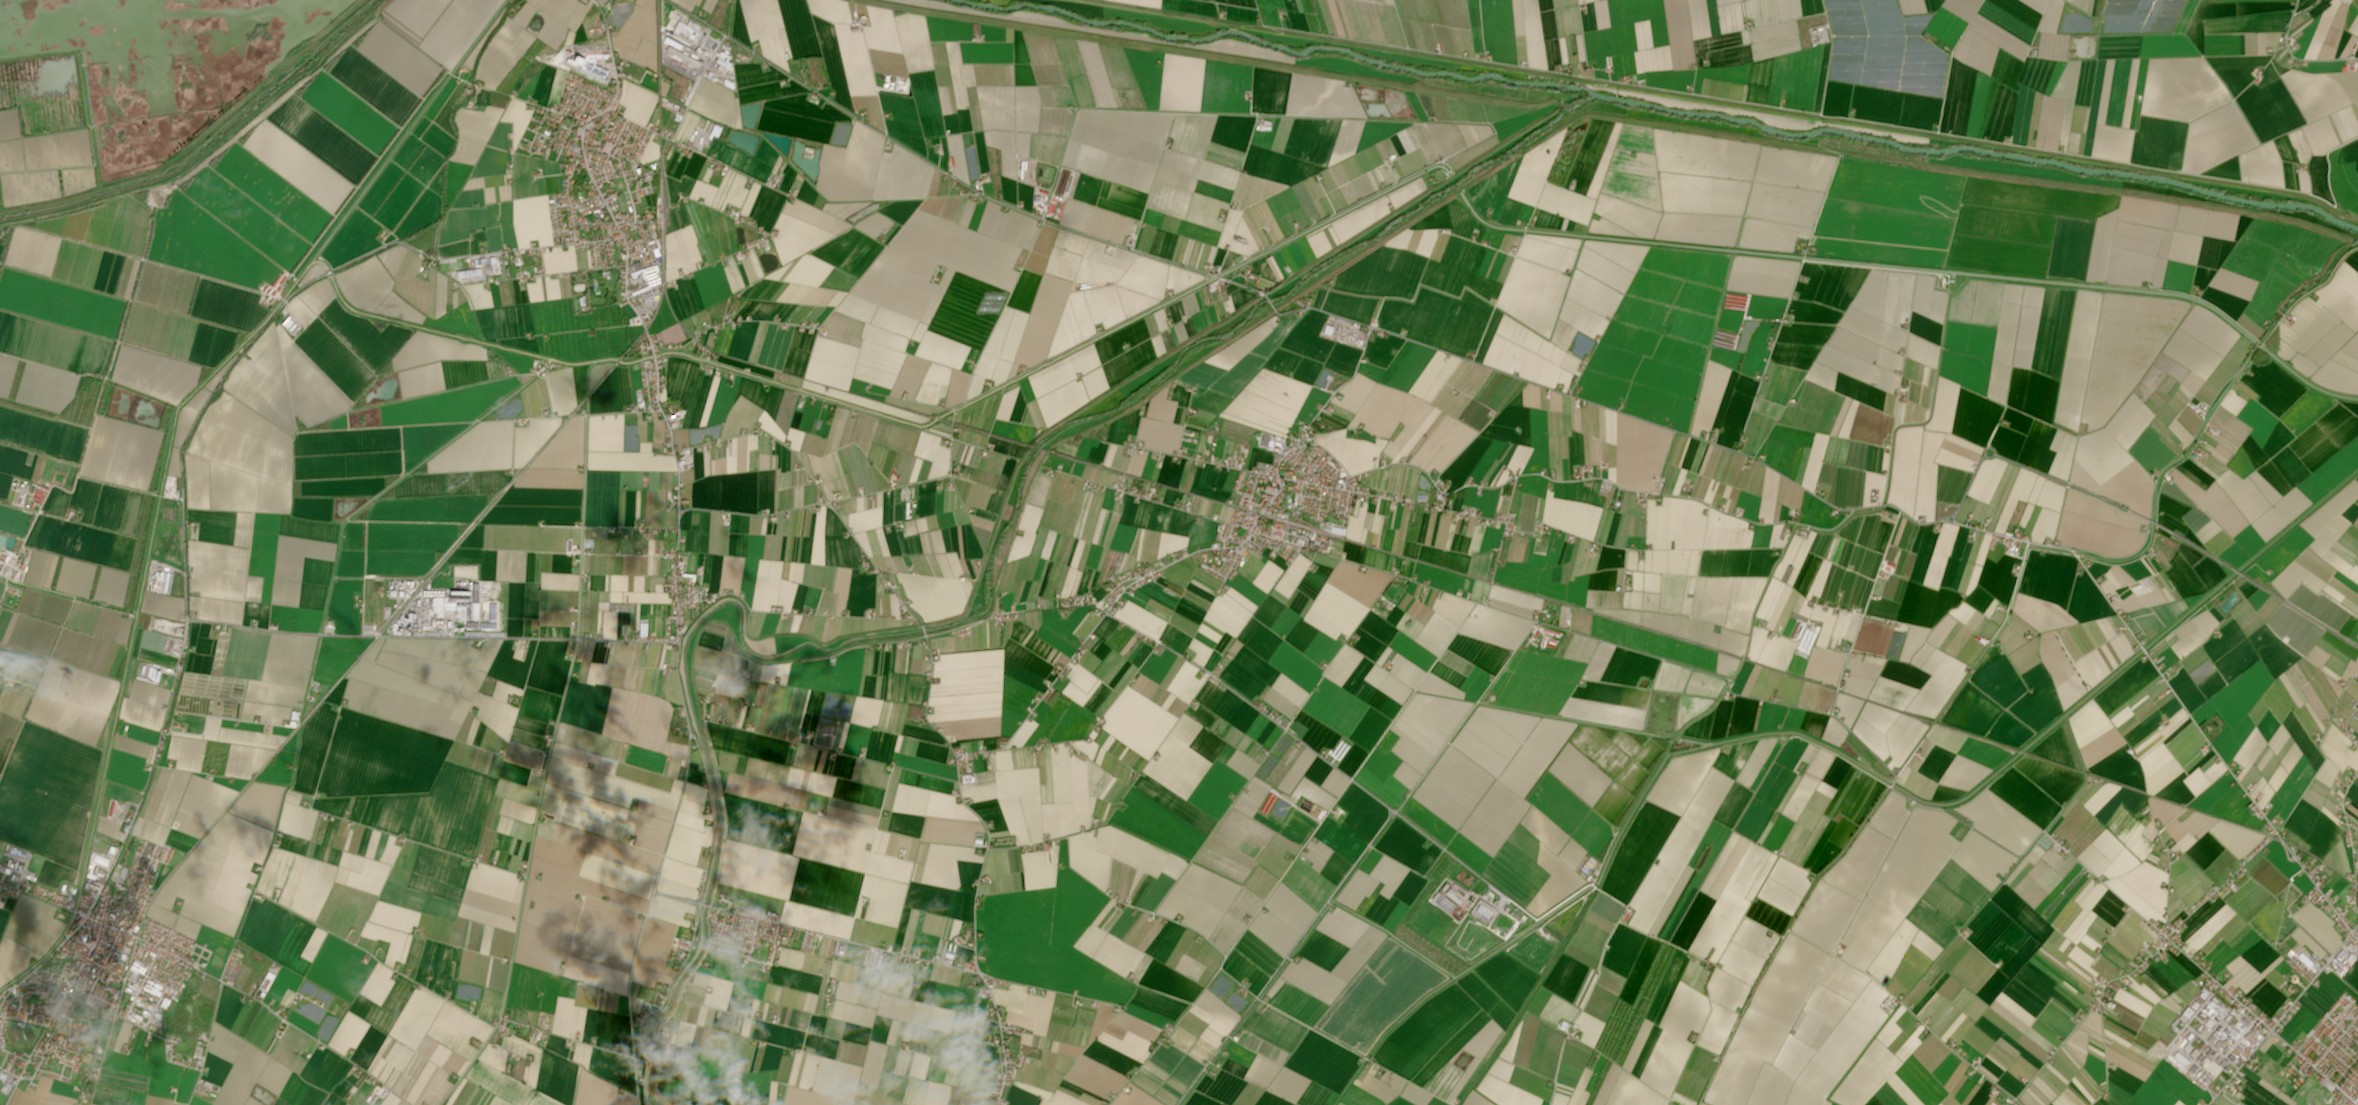
\includegraphics[width=\textwidth]{figures/2023-04-03-00_00_2023-04-03-23_59_Sentinel-2_L2A_True_color.jpg}
        \caption{Before-event true color image for Emilia-Romagna acquired on 3 April 2023.}
        \label{fig:emilia_truecolor_before}
    \end{subfigure}
    \hfill
    \begin{subfigure}[t]{0.49\textwidth}
        \centering
        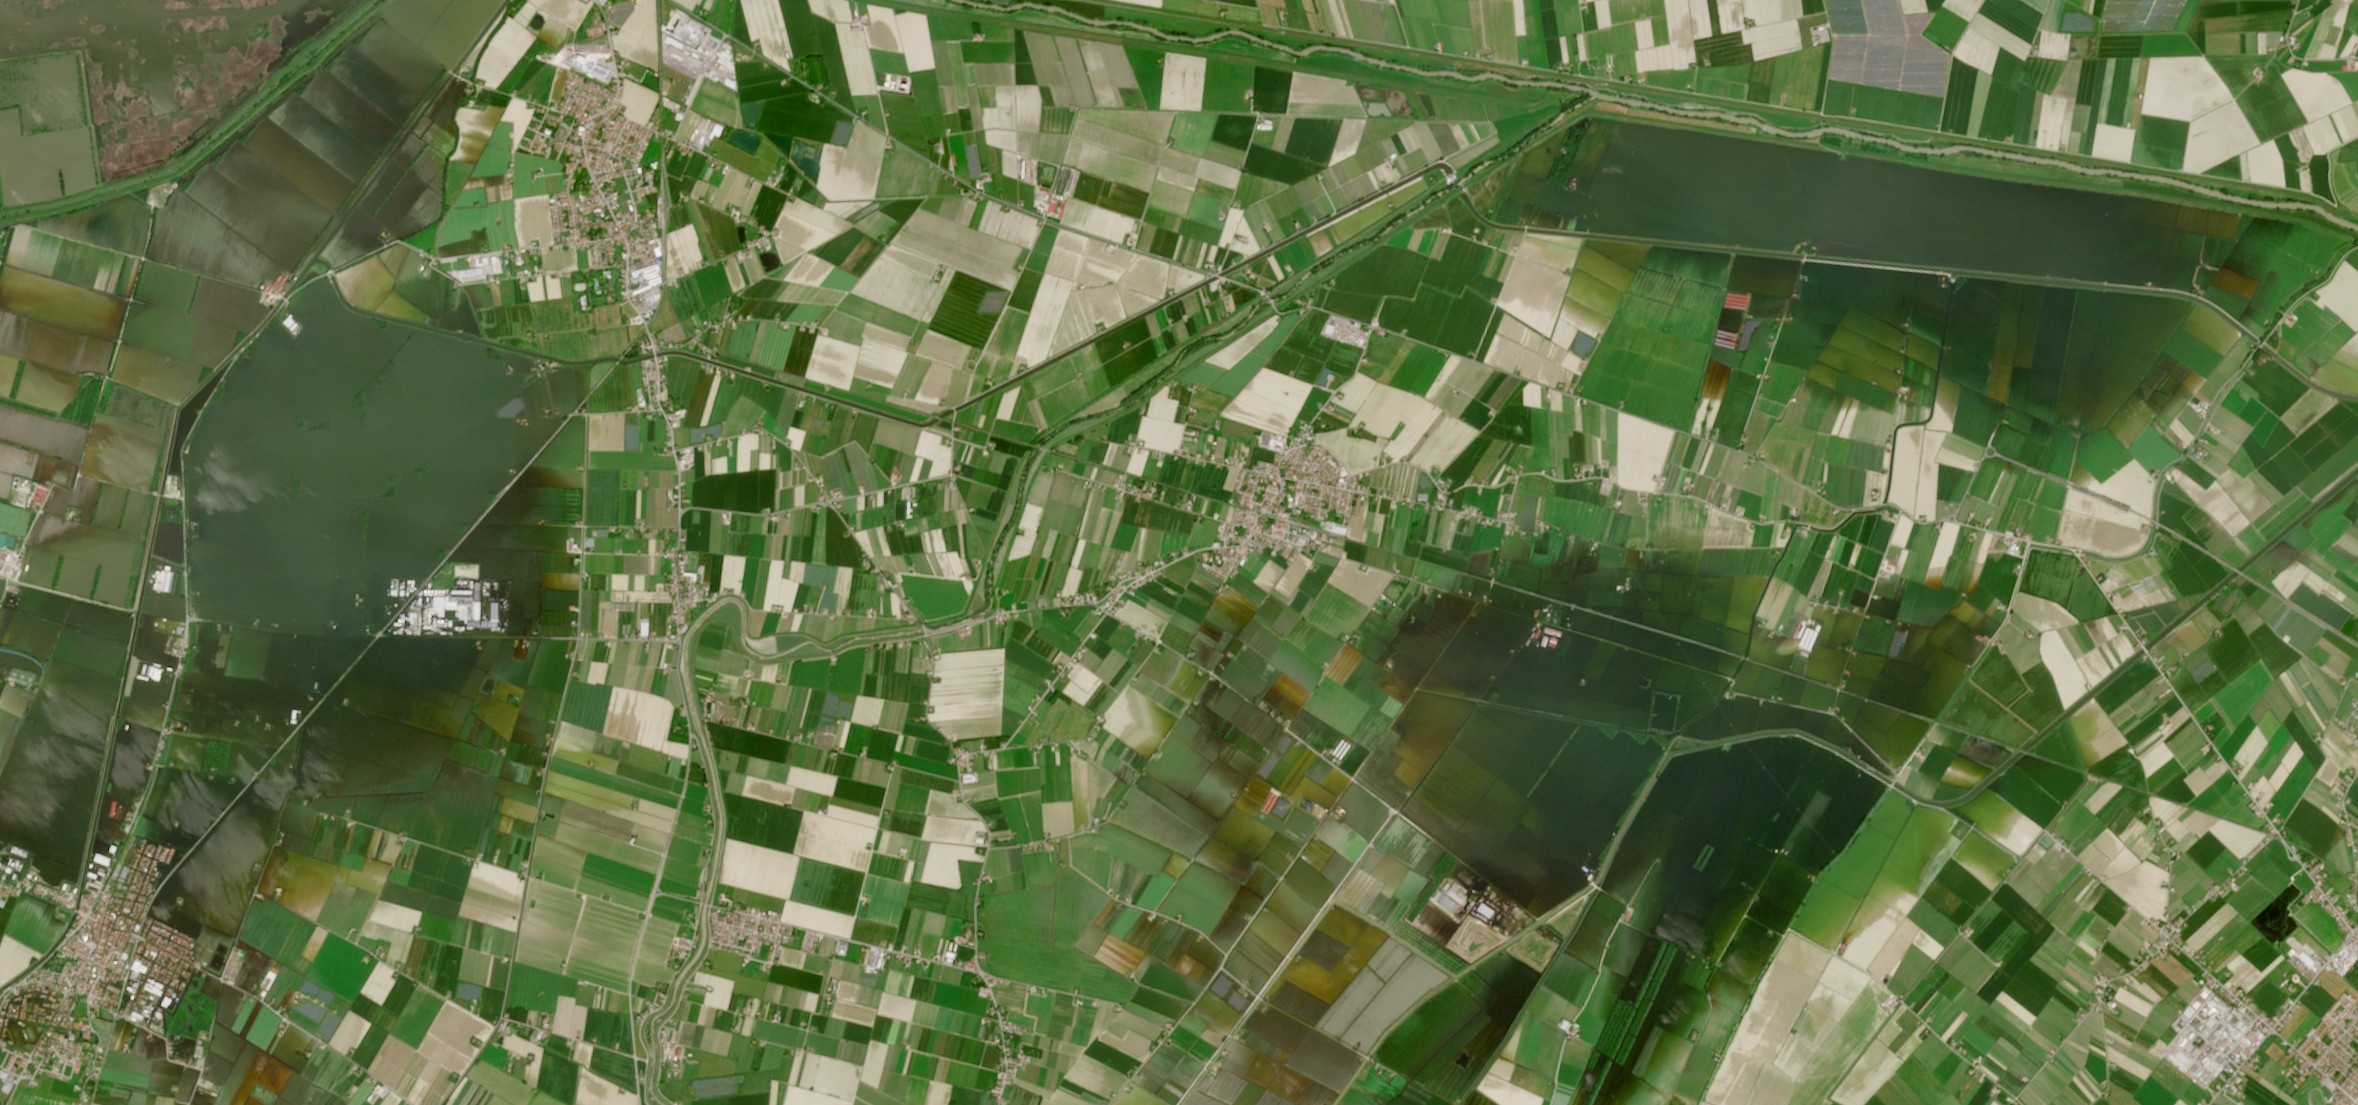
\includegraphics[width=\textwidth]{figures/2023-05-23-00_00_2023-05-23-23_59_Sentinel-2_L2A_True_color.jpg}
        \caption{After-event true color image for Emilia-Romagna acquired on 23 May 2023.}
        \label{fig:emilia_truecolor_after}
    \end{subfigure}
    \caption{Side-by-side comparison of Sentinel-2 true color imagery for the Emilia-Romagna flood case before and after the event. The comparison highlights the visible expansion of water-covered areas across the agricultural landscape.}
    \label{fig:emilia_truecolor_comparison}
\end{figure}

\begin{figure}[H]
    \centering
    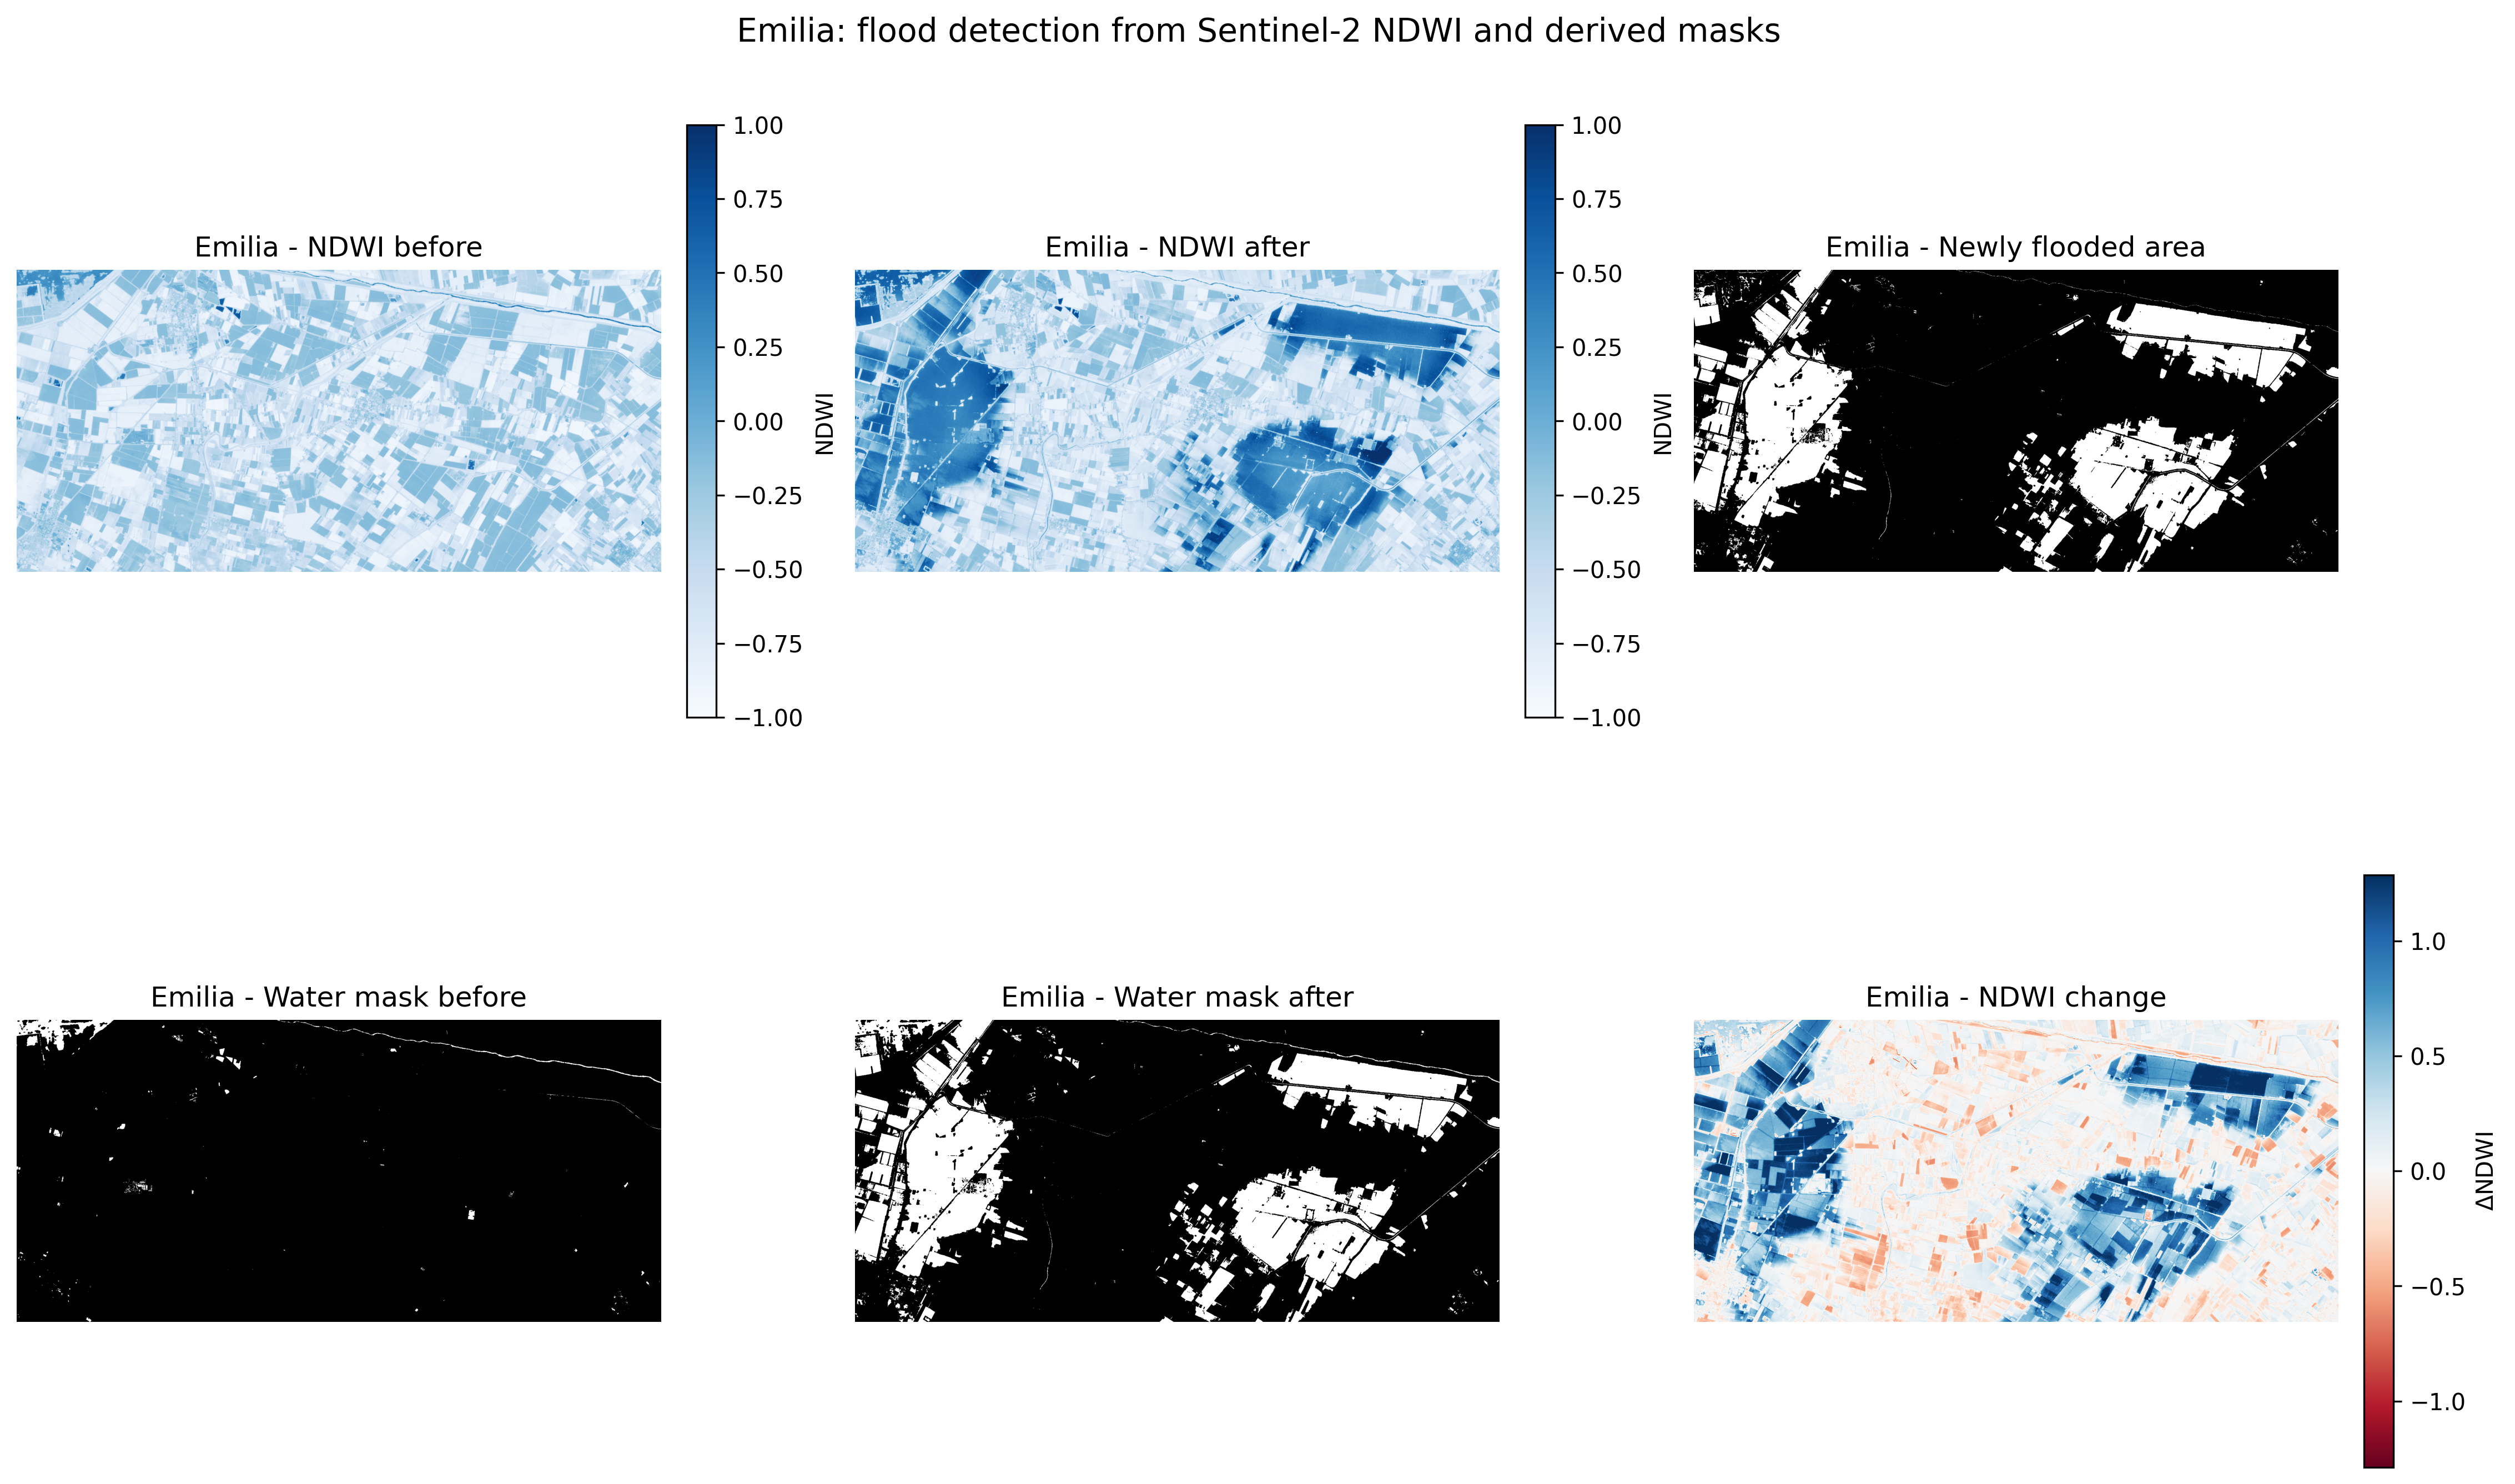
\includegraphics[width=\textwidth]{figures/Emilia_flood_report_figure.png}
    \caption{Flood detection results for Emilia-Romagna. The figure shows NDWI before and after the event, the newly flooded area mask, the water masks before and after the event, and the NDWI change map.}
    \label{fig:emilia_flood_report}
\end{figure}

\subsubsection{Wildfire Results}

\begin{table}[H]
\centering
\resizebox{\textwidth}{!}{
\begin{tabular}{lcccccc}
\toprule
Event & NDVI before & NDVI after & NDVI drop & dNBR & Veg loss (\%) & Burned area (\%) \\
\midrule
Greece & 0.4516 & 0.3257 & 0.1259 & 0.0453 & 21.0630 & 13.8515 \\
Serra da Estrela & 0.4751 & 0.3944 & 0.0807 & 0.1419 & 16.3626 & 17.4823 \\
Turkey & 0.3559 & 0.2871 & 0.0688 & -0.0763 & 14.1518 & 3.6802 \\
\bottomrule

\end{tabular}
}
\caption{Wildfire indicators derived from Sentinel-2 imagery}

\end{table}

The wildfire events show different levels of vegetation loss and burn severity. The Greece wildfire presents a strong vegetation loss and a large burned area, while the Serra da Estrela event shows a strong burn signal reflected in the dNBR value. The Turkey wildfire shows a smaller burned area, although vegetation loss is still detectable. Following we present the Turkey case.

\begin{figure}[H]
    \centering
    \begin{subfigure}[t]{0.49\textwidth}
        \centering
        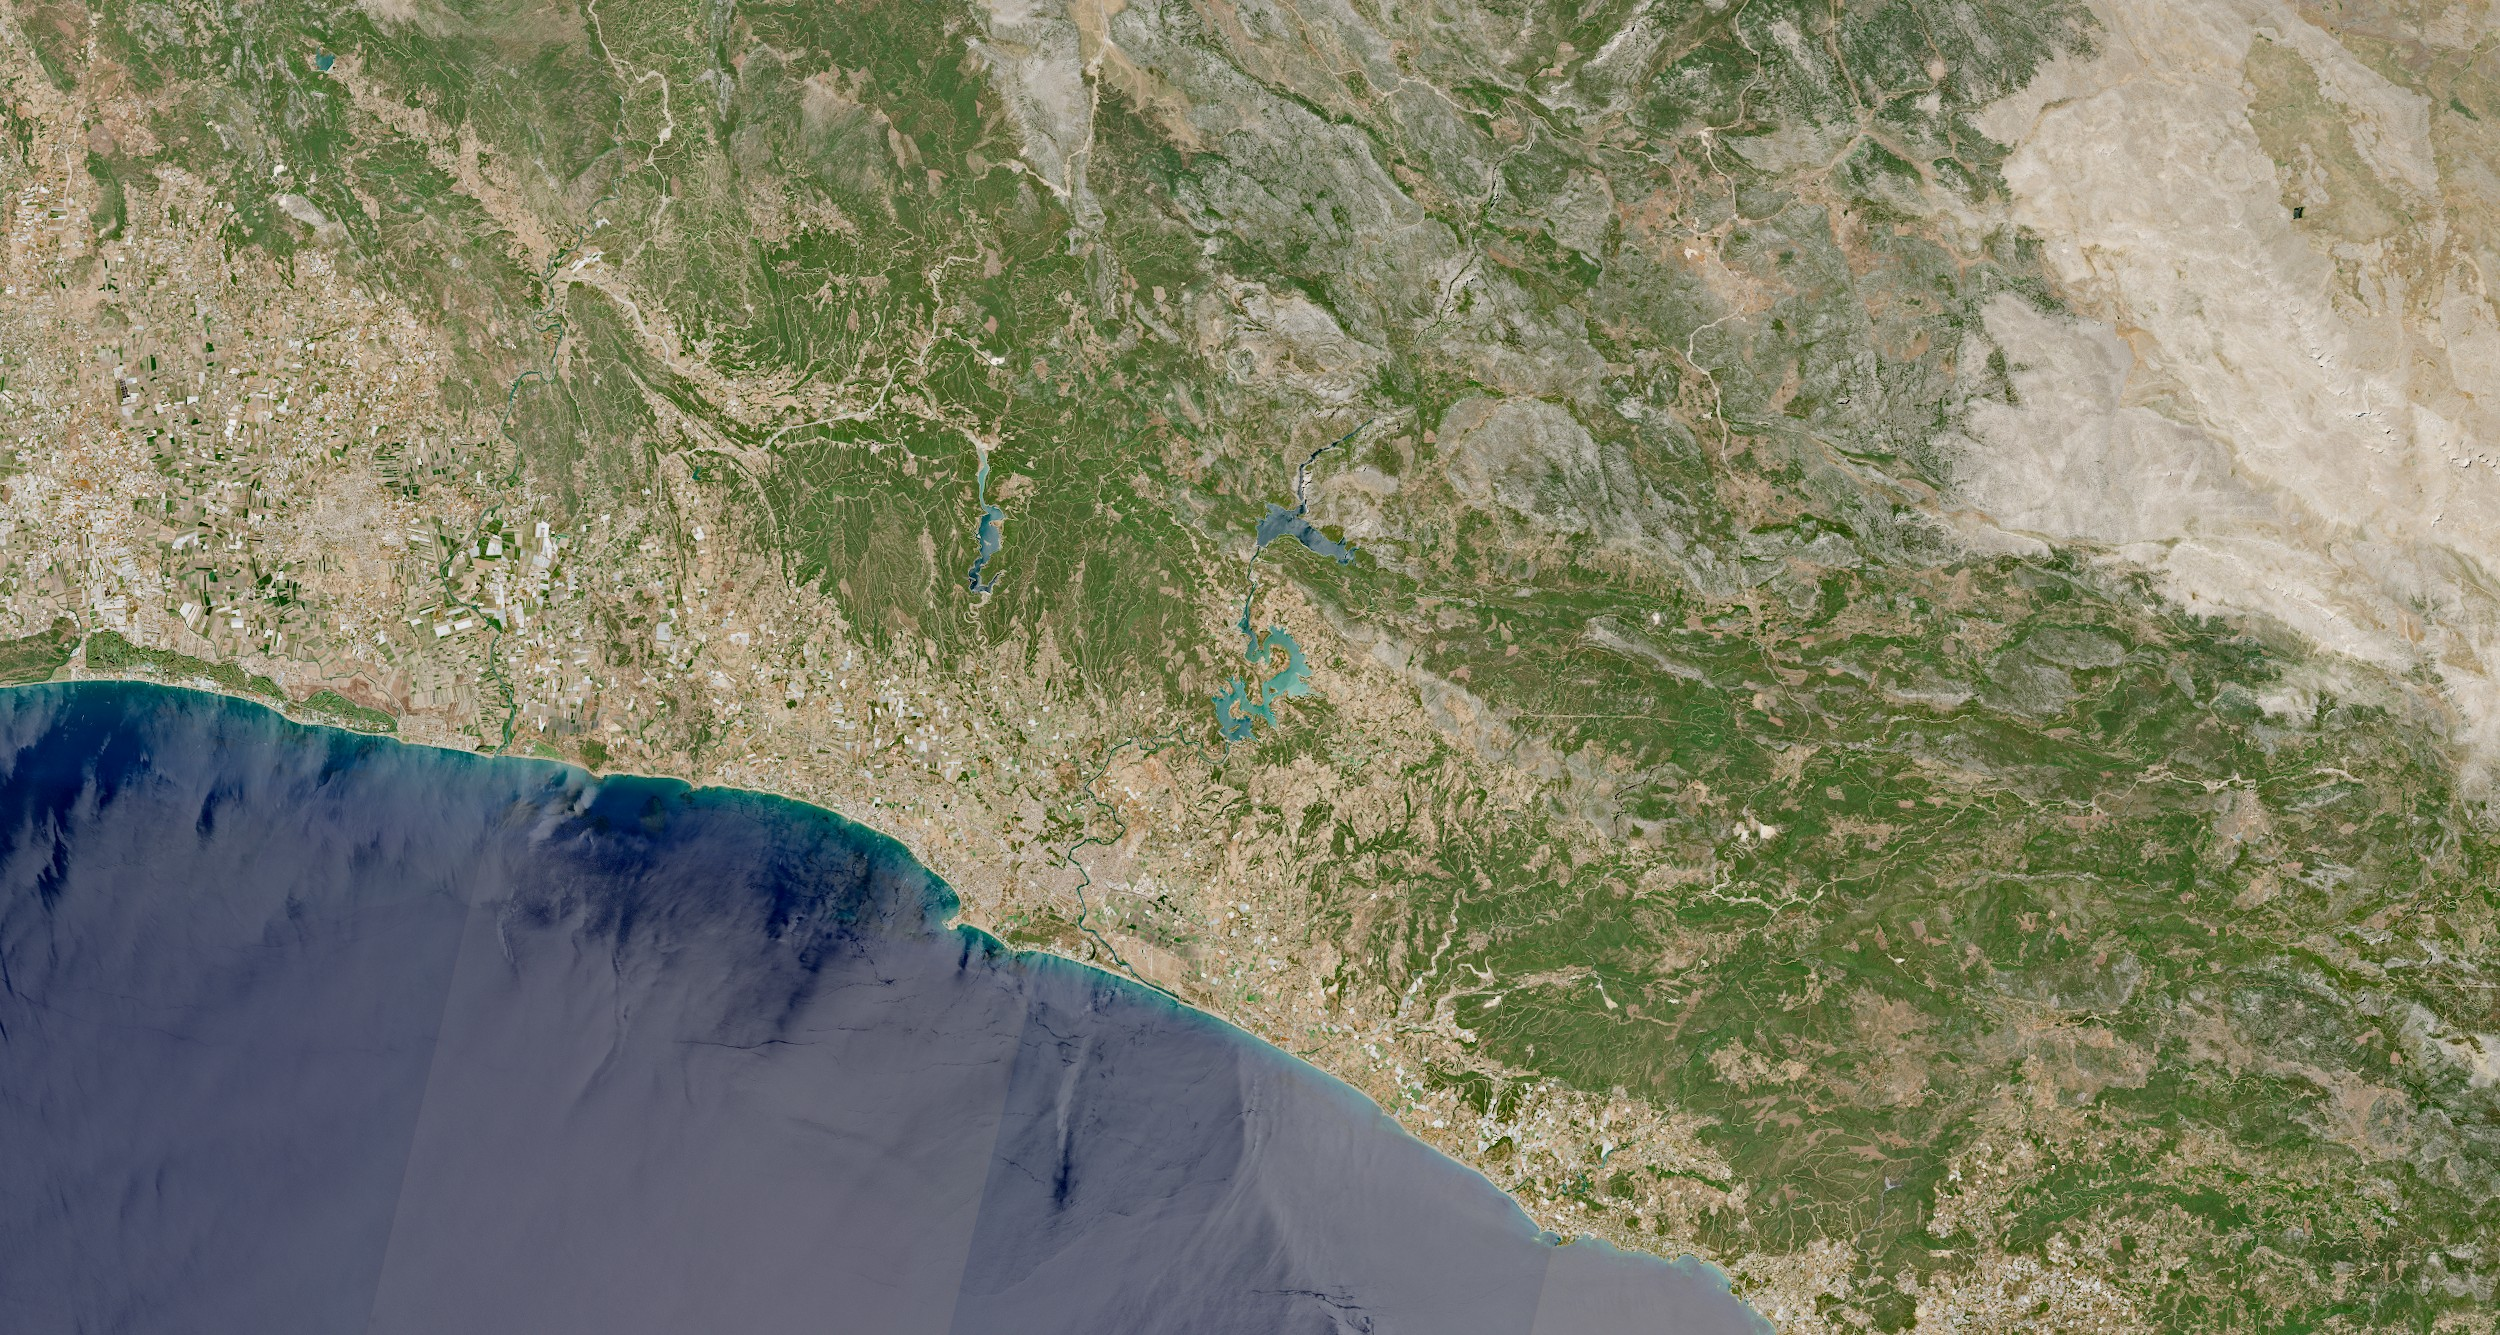
\includegraphics[width=\textwidth]{figures/2021-06-30-00_00_2021-06-30-23_59_Sentinel-2_L2A_True_color.jpg}
        \caption{Before-event true color image for the Turkey wildfire acquired on 30 June 2021.}
        \label{fig:turkey_truecolor_before}
    \end{subfigure}
    \hfill
    \begin{subfigure}[t]{0.49\textwidth}
        \centering
        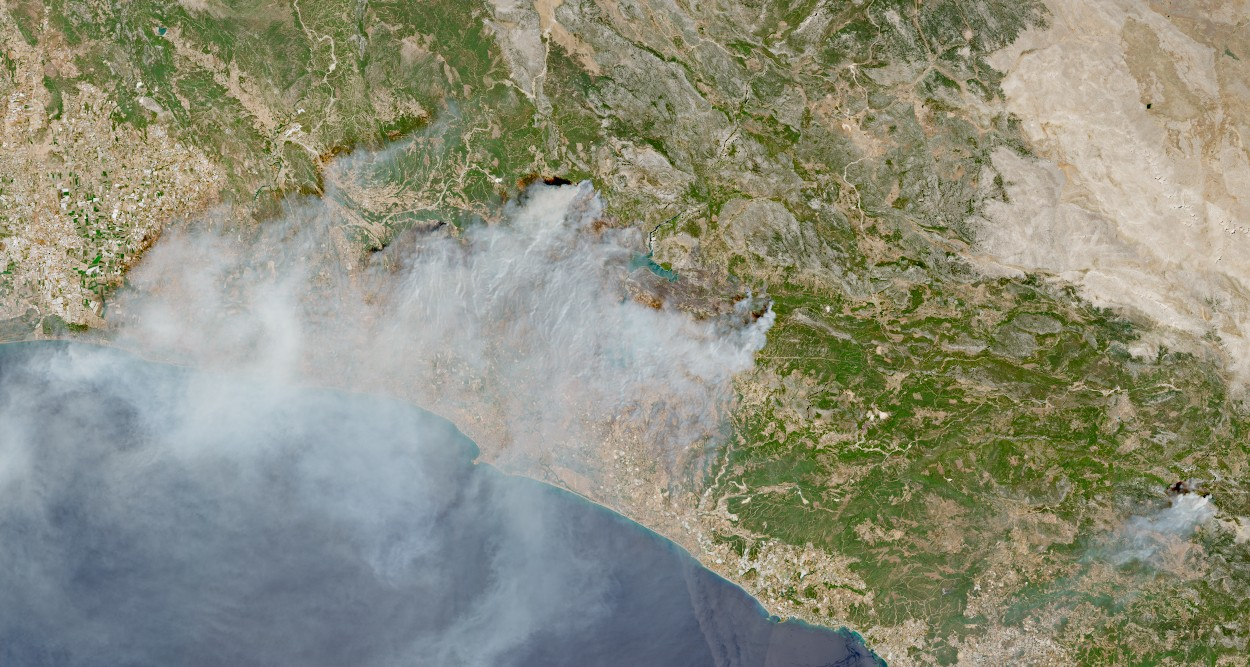
\includegraphics[width=\textwidth]{figures/2021-07-30-00_00_2021-07-30-23_59_Sentinel-2_L2A_True_color.jpg}
        \caption{After-event true color image for the Turkey wildfire acquired on 30 July 2021.}
        \label{fig:turkey_truecolor_after}
    \end{subfigure}
    \caption{Side-by-side comparison of Sentinel-2 true color imagery for the Turkey wildfire case before and after the event. The after-event image shows smoke and visibly altered surface conditions associated with the wildfire.}
    \label{fig:turkey_truecolor_comparison}
\end{figure}

\begin{figure}[H]
    \centering
    \includegraphics[width=\textwidth]{figures/Turkey_wildfire_report_figure.png}
    \caption{Wildfire detection results for Turkey. The figure shows NDVI before and after the event, dNBR, NBR before and after the event, and the derived burn mask.}
    \label{fig:turkey_wildfire}
\end{figure}

\section{Reasoning Layer}

After the EO preprocessing stage, the system enters the reasoning layer implemented in Jason. Here, numerical EO outputs are no longer treated as isolated measurements. They are transformed into symbolic beliefs, combined with contextual metadata, and interpreted through explicit reasoning rules.

This is the core layer that makes the overall system explainable. Every classification is linked to a visible belief structure, a reasoning path, and a traceable final explanation.

Figure~\ref{fig:sequence_diagram} summarizes the temporal communication flow of the symbolic multi-agent system. The CoordinatorAgent acts as the orchestration point: it dispatches event beliefs to a hazard-specialized agent, receives the resulting assessment, optionally requests clarification when the first pass remains uncertain, and then forwards the integrated symbolic output to the ExplanationAgent.

The figure also keeps the downstream NLP handoff visible so that the reasoning layer can be understood in relation to the post-processing stage.

\begin{figure}[H]
    \centering
    \fitdiagram{figures/diagram.pdf}
    \caption{System-level interaction view of the reasoning and reporting flow.}
    \label{fig:sequence_diagram}
\end{figure}

\subsection{Belief Base}

The reasoning layer is grounded in a belief base that contains four main groups of facts:

\begin{itemize}
\item \textbf{event metadata}, describing the event identity, location, temporal window, and responsible hazard agent
\item \textbf{EO indicator beliefs}, containing the satellite-derived measurements computed in the previous layer
\item \textbf{context beliefs}, such as population exposure classes and observation-quality metadata
\item \textbf{optional user-input beliefs}, currently used to store an optional user-provided severity expectation for post-hoc comparison with the MAS conclusion
\end{itemize}

In the current implementation, the EO indicator beliefs and population exposure beliefs are generated automatically from the processed CSV outputs. The MAS therefore consumes generated \texttt{.asl} belief files rather than hand-copied numerical facts.

\subsubsection{Event Metadata Beliefs}

Each event is represented through a set of symbolic facts that specify geographic context, dates, hazard type, and temporal reliability. These beliefs are not only descriptive: they also support later caveat reasoning.\\ For instance, the beliefs \texttt{timeline\_confidence/2}, \texttt{late\_observation\_flag/2}, and \texttt{possible\_underestimation/2} are used to qualify conclusions when the post-event image may not capture the peak hazard signal.

In other words, event metadata are not just labels attached to a case. They also influence how the later reasoning stages qualify uncertainty and possible underestimation.

\begin{lstlisting}
event(ahr_valley).
name(ahr_valley, "Ahr Valley").
country(ahr_valley, germany).
region(ahr_valley, rhineland_palatinate).
event_type(ahr_valley, flood).
agent_responsible(ahr_valley, water_agent).
before_date(ahr_valley, "2021-03-30").
after_date(ahr_valley, "2021-07-21").
timeline_confidence(ahr_valley, confirmed).
late_observation_flag(ahr_valley, true).
possible_underestimation(ahr_valley, true).
\end{lstlisting}

The same representation is used for wildfire events, with the only difference being the hazard type and the assigned hazard-specialized agent.

\subsubsection{EO Indicator Beliefs}

The EO indicators extracted from Sentinel-2 imagery are encoded as logical beliefs. This makes the numerical evidence directly accessible to Jason rules.

Flood events are represented through NDWI-based change indicators:

\begin{lstlisting}
mean_ndwi_before(emilia, -0.5065).
mean_ndwi_after(emilia, -0.3007).
ndwi_change(emilia, 0.2057).
water_increase_pct(emilia, 22.73).
newly_flooded_area_pct(emilia, 22.90).
\end{lstlisting}

Wildfire events are represented through vegetation-loss and burn-related indicators:

\begin{lstlisting}
mean_ndvi_before(evros, 0.4516).
mean_ndvi_after(evros, 0.3257).
ndvi_drop(evros, 0.1259).
mean_dnbr(evros, 0.0453).
vegetation_loss_pct(evros, 21.06).
burned_area_pct(evros, 13.85).
\end{lstlisting}

\subsubsection{Context Beliefs}

The belief base also contains contextual information used during fusion. In particular, each event is associated with a population exposure class derived from WorldPop data~\cite{worldpop2025}.

These contextual beliefs are not hazard claims by themselves. They are used by the coordinator to combine hazard evidence with exposure and derive the final integrated concern profile.

\begin{lstlisting}
population_exposure_class(sindh, high).
population_exposure_class(emilia, medium).
population_exposure_class(evros, low).
\end{lstlisting}

This additional symbolic context matters because the system does not stop at hazard detection. It also reasons about how strong the case is, how much confidence should be attached to it, and how severe the situation becomes once hazard evidence is combined with exposure.

\subsubsection{Optional User-Input Beliefs}

The current architecture also supports an optional user-provided assessment entered through the UI. This information does not drive the hazard reasoning itself.

Instead, it is represented as a separate symbolic input that the coordinator compares against the inferred result after reasoning has finished.

\begin{lstlisting}
user_assessment(ahr_valley, severe).
\end{lstlisting}

This preserves the distinction between evidence-driven inference and user expectation. The hazard agents still infer the case only from EO and contextual beliefs, while the optional user assessment becomes part of the final explanation only as a comparison signal.

\subsection{Hazard-Specific Symbolic Reasoning}

Two specialized agents perform hazard interpretation: \texttt{forest\_agent} for wildfire cases and \texttt{water\_agent} for flood cases.

Both agents follow the same general pattern. They start from raw EO indicator beliefs, derive intermediate evidence predicates, select a severity path, assign a confidence label, derive an explicit conclusion status, and finally generate caveats. In the current version, they also support a second-pass clarification stage that can be triggered by the coordinator for uncertain or caveat-heavy cases.

\subsubsection{Wildfire Reasoning in \texttt{forest\_agent}}

The wildfire agent reasons in layers rather than applying a single threshold. First, raw indicators activate evidence predicates such as vegetation damage, burn extent, and spectral burn support.\\

These predicates are then combined into more abstract patterns such as coherent evidence, mixed evidence, or strong multisignal evidence.

\begin{lstlisting}
vegetation_damage_signal(E) :-
    vegetation_loss_pct(E, VegetationLoss) &
    VegetationLoss >= 12.

burn_extent_signal(E) :-
    burned_area_pct(E, BurnedArea) &
    BurnedArea >= 3.

spectral_burn_signal(E) :-
    mean_dnbr(E, MeanDNBR) &
    MeanDNBR >= 0.04.

strong_multisignal_fire_evidence(E) :-
    strong_vegetation_damage(E) &
    strong_burn_extent(E) &
    strong_spectral_burn_signal(E).
\end{lstlisting}

Once the evidence pattern is known, the agent selects a specific severity rule. The rule stores not only the final label, but also the symbolic claim label, the evidence list that supported the conclusion, and the name of the rule that was activated.\\

\begin{lstlisting}
fire_severity_path(E, severe, strong_multisignal_fire_damage,
    [vegetation_loss_pct, burned_area_pct, mean_dnbr],
    rule_severe_fire_multisignal) :-
    strong_multisignal_fire_evidence(E).
\end{lstlisting}

This design makes the reasoning path explicit. For example, the system can distinguish between a wildfire case supported by vegetation loss and burned area, a case supported mainly by burn extent and dNBR, and a weaker case supported only by NDVI variation.\\

Confidence is then derived from the overall quality of support, while caveats are attached when the evidence is mixed or temporally uncertain.

In the current implementation, inconclusive cases are represented explicitly in the MAS rather than being verbalized only at report time.

When the available signals do not support a reliable hazard conclusion, the agents produce an \texttt{undetermined} severity together with an explicit \texttt{inconclusive} conclusion status.

\subsubsection{Support-Level Abstraction}

The current version of the reasoning layer introduces an intermediate symbolic abstraction between evidence synthesis and final decision. Rather than mapping evidence patterns directly to severity and confidence, the hazard agents first classify the available evidence in terms of support level.

The main symbolic categories are:

\begin{itemize}
\item \texttt{strong}, for consistent multisignal evidence
\item \texttt{moderate}, for coherent but not fully reinforced evidence
\item \texttt{weak}, for limited or residual evidence
\item \texttt{conflicting}, for partially contradictory evidence
\item \texttt{insufficient}, for cases in which no reliable hazard-support pattern can be established
\end{itemize}

This layer separates \emph{evidence interpretation} from \emph{decision output}. Severity and confidence are therefore no longer derived as a single jump from thresholds to labels.

Instead, the agents first construct a symbolic judgment about how strongly the evidence supports the hazard hypothesis, and only then map that support level into severity, confidence, and conclusion status.

\subsubsection{Flood Reasoning in \texttt{water\_agent}}

The flood agent uses an analogous reasoning structure. It starts from \texttt{water\_increase\_pct/2}, \texttt{newly\_flooded\_area\_pct/2}, and \texttt{ndwi\_change/2}, and converts them into symbolic flood evidence.

Figure~\ref{fig:water_agent_diagram} details the internal communication and reasoning flow of the \texttt{water\_agent}. Unlike the previous higher-level diagrams, this figure expands the internal symbolic stages explicitly, from indicator-level signals to evidence-pattern construction, support-level assignment, severity-path selection, caveat derivation, and clarification handling.

\begin{figure}[H]
    \centering
    \fitdiagram{figures/waterdiagram.pdf}
    \caption{Detailed communication and reasoning flow for the \texttt{water\_agent}.}
    \label{fig:water_agent_diagram}
\end{figure}

\begin{lstlisting}
water_expansion_signal(E) :-
    water_increase_pct(E, WaterIncrease) &
    WaterIncrease >= 8.

flood_extent_signal(E) :-
    newly_flooded_area_pct(E, NewlyFlooded) &
    NewlyFlooded >= 8.

ndwi_shift_signal(E) :-
    ndwi_change(E, NdwiChange) &
    NdwiChange >= 0.08.

coherent_flood_evidence(E) :-
    water_expansion_signal(E) &
    flood_extent_signal(E) &
    ndwi_shift_signal(E).
\end{lstlisting}

The flood agent is also able to represent residual or weak flood signals. This is especially relevant for cases such as Ahr Valley, where the post-event image was acquired several days after the flood peak.

In these situations, the system does not force a strong hazard conclusion. Instead, it can derive either a residual signal qualified by caveats, or an explicit inconclusive outcome when the evidence is insufficient to support a reliable hazard classification.

\begin{lstlisting}
flood_severity_path(E, mild, residual_flood_signal,
    [water_increase_pct, newly_flooded_area_pct],
    rule_residual_flood_late_observation) :-
    residual_flood_evidence(E).
\end{lstlisting}

As in the wildfire case, the output of the hazard agent is not a single label but a structured symbolic assessment:

\begin{lstlisting}
hazard_assessment(E, Hazard, Severity, SupportLevel, ConclusionStatus,
    ConfidenceLevel, ClaimLabel, PrimaryCaveat, EvidenceList,
    CaveatList, RuleLabel)
\end{lstlisting}

\subsubsection{Specialist Clarification Stage}

The hazard agents now have a second role in addition to first-pass classification. When the coordinator judges that a case is uncertain, the same specialist agent is asked to clarify its own assessment rather than delegating the case to a different domain agent.

This preserves specialization while introducing a genuine cooperative loop.

The clarification step is implemented through a second achievement goal:

\begin{lstlisting}
clarify_assessment(E, ClaimLabel, PrimaryCaveat, Requester)
\end{lstlisting}

The specialist then returns a structured symbolic clarification object containing:

\begin{itemize}
\item the main limitation affecting the first-pass interpretation
\item the strongest retained evidence
\item an optional alternative claim
\item the clarification status
\end{itemize}

\begin{lstlisting}
clarification_result(E, ClaimLabel, PrimaryLimitation,
    StrongestEvidence, AlternativeClaim, ClarificationStatus)
\end{lstlisting}

The result is that the architecture is no longer only a linear pipeline. In straightforward cases, the specialist produces a first-pass judgment and the system proceeds directly to fusion.

In uncertain cases, the coordinator requests a second symbolic refinement from the same specialist before finalizing the case.

\subsection{Coordinator Fusion}

The coordinator performs two distinct tasks: orchestration and fusion.

The \texttt{coordinator\_agent} first scans all \texttt{event/1} beliefs, checks \texttt{agent\_responsible/2}, and sends the goal \texttt{assess\_event(E, coordinator\_agent)} to the relevant hazard agent.

When a \texttt{hazard\_assessment(...)} message is received, the coordinator stores several derived beliefs. In particular, it records the hazard result, a hazard trace, and a set of \texttt{claim\_support/4} facts that make the provenance of each symbolic conclusion explicit.

\begin{lstlisting}
+hazard_result(E, Hazard, Severity, HazardConfidence,
    ClaimLabel, PrimaryCaveat, SourceAgent);
+hazard_trace(E, SourceAgent, RuleLabel, EvidenceList, CaveatList);
+claim_support(E, hazard_classification, SourceAgent, EvidenceList);
\end{lstlisting}

Before fusion, the coordinator checks whether the first-pass output should be accepted directly or whether it requires a clarification round. This decision is based on the confidence level and on specific caveat labels rather than on any external gold label.

In the current implementation, clarification is requested for low-confidence cases and for selected medium-confidence cases associated with caveats such as \texttt{burn\_signal\_weak}, \texttt{weak\_water\_signal}, \texttt{residual\_observation\_window}, or \texttt{limited\_multisignal\_support}.

\begin{lstlisting}
clarification_required(low, _).
clarification_required(medium, burn_signal_weak).
clarification_required(medium, weak_water_signal).
clarification_required(medium, residual_observation_window).
\end{lstlisting}

If clarification is required, the coordinator stores a temporary \texttt{clarification\_context(...)} belief, sends a clarification request back to the same specialist, and waits for a \texttt{clarification\_result(...)} reply.

Only after that does it proceed to the fusion step.

The coordinator then combines hazard output with population exposure and caveat-aware confidence rules to derive an integrated symbolic case.

Four derived predicates are central in this step:

\begin{itemize}
\item \texttt{concern\_level/3}, combining hazard severity and exposure
\item \texttt{fusion\_confidence/4}, adjusting hazard confidence using the primary caveat
\item \texttt{interpretation\_mode/3}, determining whether the reading is robust, qualified, cautious, or tentative
\item \texttt{case\_profile/4}, producing a compact integrated label such as \texttt{high\_priority\_event}
\end{itemize}

\begin{lstlisting}
population_exposure_class(E, ExposureClass);
concern_level(Severity, ExposureClass, ConcernLevel);
fusion_confidence(Severity, HazardConfidence, PrimaryCaveat, FusionConfidence);
interpretation_mode(FusionConfidence, PrimaryCaveat, InterpretationMode);
case_profile(ConcernLevel, FusionConfidence, InterpretationMode, Profile);
\end{lstlisting}

The integrated case now also records whether clarification occurred and, if so, which limitation and strongest evidence were returned by the specialist.

As a result, the final interpretation is not based only on EO measurements. It also depends on contextual exposure, on the reliability of the hazard reading, and on whether the case required a second-pass refinement. A severe flood in a high-exposure area and a mild wildfire in a low-exposure area are therefore represented differently even if both originate from the same general reasoning architecture.

The coordinator also stores the conclusion status returned by the specialist and, when available, compares the final inferred severity with the optional \texttt{user\_assessment/2} belief provided through the UI.

This comparison does not modify the reasoning result. It is used only to expose alignment or disagreement in the final explanation.

\subsection{Threshold Design and Limitations}

The thresholds used in the hazard agents should be understood as interpretable prototype cutoffs rather than as operational EO standards. In the current implementation, they were not introduced as arbitrary constants. Instead, they were chosen as literature-informed heuristic ranges and then tuned against the small case-study dataset used in this project so that the symbolic layer could separate strong, moderate, weak, conflicting, residual, and inconclusive patterns in a readable way.

More precisely, the thresholds are intended to:

\begin{itemize}
\item reflect typical relative ranges discussed for EO-derived water, vegetation, and burn indicators, without claiming to be universal remote-sensing thresholds
\item align the symbolic rules with qualitative EO interpretation found in the scientific literature, for example that stronger flood or burn evidence should require larger and more coherent changes across multiple indicators
\item remain separable on the small case-study set used in this prototype, so that the rule base can distinguish strong multisignal cases from weaker or residual ones
\item separate strong multisignal cases from coherent but weaker cases
\item isolate residual, weak, or contradictory situations that should trigger caveats or clarification
\item keep the reasoning layer transparent and easy to inspect
\end{itemize}

This design choice improves interpretability, but it also introduces clear limitations. The current reasoning layer remains dependent on manually defined cutoffs, is sensitive to indicator noise and case-specific edge conditions, and has not been calibrated on a large benchmark dataset. The thresholds should therefore be interpreted as scientifically motivated symbolic design choices rather than as validated operational standards. These limitations are acceptable within the goals of the project, which focus on symbolic reasoning, explainability, and controlled demonstration rather than on operational large-scale deployment.

\subsection{Explanation Generation and Traceability}

The final stage of the reasoning layer is handled by the \texttt{explanation\_agent}. This agent does not inspect raw EO indicators directly.

Instead, it receives the integrated symbolic case generated by the coordinator together with the rule label, evidence list, caveat list, and clarification metadata coming from the previous stages.

In the current architecture, the explanation agent is no longer the final natural-language generator. Its role is to package the integrated symbolic case into a structured semantic artifact that can later be exported to Python and reused by the ontology and reporting components.

The explanation payload preserves:

\begin{itemize}
\item event identity and geographic metadata
\item hazard, severity, conclusion status, concern, confidence, and case profile
\item claim label, evidence list, and caveat structure
\item clarification status, strongest evidence, and alternative claim
\item provenance information such as source agent and rule label
\item optional user-assessment alignment metadata
\item an explicit \texttt{explanation\_trace(...)}
\end{itemize}

\begin{lstlisting}
semantic_explanation(E,
    event_frame(...),
    assessment_frame(...),
    evidence_frame(...),
    clarification_frame(...),
    provenance_frame(...),
    headline_frame(...),
    debug_text(...),
    explanation_trace(...))
\end{lstlisting}

This trace preserves the provenance of the final explanation package. The semantic payload is therefore not a detached summary: it is grounded in the exact symbolic rule that fired, the evidence predicates that supported the claim, the caveats that qualified the interpretation, and the clarification status associated with the case.

The coordinator also exports this payload as raw Jason JSON, so the downstream Python layer can consume it without redoing the symbolic reasoning.

\subsection{Conditional Cooperation}

The current architecture can therefore be described as a \textbf{rapid specialist MAS with conditional clarification}. It is not a negotiation-heavy MAS in which every agent comments on every event. Instead, it uses two stages:

\begin{enumerate}
\item a fast first-pass specialist assessment
\item a second-pass clarification loop activated only for uncertain or caveat-heavy cases
\end{enumerate}

For hazard assessment, this design keeps most cases quick and transparent while allowing only ambiguous cases to trigger additional interaction.

The result is a system that remains specialized and efficient, but is also more cooperative than a simple one-way pipeline.

\subsection{Role of the Reasoning Layer}

The reasoning layer is the component that turns EO indicators into explainable environmental interpretations. Its contribution is not limited to classifying wildfire and flood events. It explicitly represents:

\begin{itemize}
\item which beliefs are stored for each event
\item which indicator thresholds activate symbolic evidence
\item which severity path is selected by each hazard agent
\item which caveats reduce or qualify confidence
\item when the coordinator triggers a second-pass clarification request
\item how the coordinator fuses hazard output with population exposure
\item how the final explanation exposes whether clarification was required
\item how the final explanation is linked to a symbolic trace
\end{itemize}

\section{NLP Layer}

After the Jason reasoning layer has produced a \texttt{semantic\_explanation(...)} structure, the system enters a Python-based post-processing pipeline. This layer is not responsible for hazard reasoning itself. Its function is to take the symbolic output generated by Jason, normalize it into a more usable semantic representation, instantiate the ontology, and finally produce readable reports.

The NLP layer is therefore better understood as a \textbf{semantic transformation and explanation delivery layer} rather than as a second reasoning engine. More precisely, the Python pipeline does not read raw hazard beliefs directly from the specialists. It receives the already-packaged semantic artifact produced by the \texttt{explanation\_agent}, which acts as the bridge between the symbolic reasoning layer and the downstream ontology and reporting components.

The pipeline is implemented as a sequence of Python modules coordinated by a single execution script. Conceptually, the flow is:

\begin{center}
raw Jason JSON $\rightarrow$ transformed semantic JSON $\rightarrow$ populated ontology $\rightarrow$ English report
\end{center}

This stage has three main responsibilities:

\begin{enumerate}
\item transform the raw Jason JSON export into a cleaner semantic JSON representation
\item populate the EO2Explain ontology from that transformed representation
\item generate readable event reports in English
\end{enumerate}

\subsection{Transformation of Jason Output}

The first step is carried out by a transformer module that reads the raw JSON exported from Jason. This export corresponds to the \texttt{semantic\_explanation(...)} payload assembled by the \texttt{explanation\_agent}.

It is structurally faithful to Jason terms, but it is still too close to the internal symbolic representation. Each payload is expressed through nested \texttt{functor}, \texttt{predicate}, and \texttt{terms} fields, which are useful for preserving symbolic structure but inconvenient for later querying and reporting.

The transformer therefore performs a semantic flattening step. It decodes Jason terms, unwraps nested frames, converts atomic symbolic labels into plain strings, and produces a cleaner schema organised into explicit sections such as:

\begin{itemize}
\item \texttt{event}
\item \texttt{assessment}
\item \texttt{evidence}
\item \texttt{clarification}
\item \texttt{provenance}
\item \texttt{headline}
\item \texttt{debug}
\item \texttt{trace}
\end{itemize}

This transformed JSON is the real interface between the MAS and the downstream explanation components. It preserves the semantics of the original symbolic explanation while making the payload easier to consume programmatically.

For example, rather than navigating raw Jason term objects, later modules can directly access fields such as \texttt{assessment.claim\_label}, \texttt{evidence.evidence\_items}, or \texttt{provenance.rule\_label}.

In the current implementation, the transformed assessment structure also preserves the MAS-derived \texttt{conclusion\_status}. This is important because report generation and ontology population must distinguish between a true hazard classification and an explicitly inconclusive outcome that was already reasoned about by the agents.

\subsection{Ontology Population}

The second step is ontology population. The current implementation uses \texttt{Owlready2} to load the base EO2Explain ontology and instantiate it automatically from the transformed semantic JSON.

This is an important design choice because the ontology is not treated as a static modeling artifact created only in Prot\'eg\'e. Instead, it becomes an executable semantic layer populated directly from the MAS output.

For each analyzed event, the population script creates or updates ontology individuals corresponding to:

\begin{itemize}
\item the event itself
\item its assessment
\item the supporting evidence bundle
\item the clarification object
\item the provenance record
\item the explanation trace
\end{itemize}

In addition, the script also creates or reuses shared semantic individuals for hazards, severity levels, confidence levels, exposure levels, concern levels, caveats, evidence items, agents, rules, and claim labels. The populated ontology also stores the MAS-derived \texttt{conclusion\_status} and \texttt{support\_level} as assessment data properties.

This allows the ontology to capture both event-specific structures and reusable controlled vocabulary terms while remaining aligned with the current symbolic reasoning model.

The resulting ontology therefore represents not only the final decision, but also how that decision was constructed. An event is linked to an assessment; the assessment is linked to its evidence bundle, clarification, and provenance; and the explanation trace acts as a structured summary layer that connects the semantic components later used by the validation, querying, and reporting stages.

In this sense, the ontology functions as an active semantic layer after population rather than as a passive representation artifact.

The ontology is not only exported as a passive artifact. After population, the Python layer now uses it in two concrete ways:

\begin{itemize}
\item \textbf{semantic validation}: a post-population checker verifies structural constraints such as one assessment per event, exactly one severity/support/conclusion-status value per assessment, and basic consistency conditions such as the exclusion of high confidence for explicitly inconclusive cases
\item \textbf{structured querying}: a lightweight query stage derives summaries such as all severe floods, all low-confidence cases, all clarification cases, and all weak/conflicting support cases
\end{itemize}

This makes the ontology an active post-MAS semantic layer rather than a decorative export.

\subsection{Report Generation}

The third step is report generation. A dedicated Python generator reads the transformed semantic JSON and converts it into readable English text.

In practical terms, the final report is therefore generated from the explanation package originally created by the \texttt{explanation\_agent}, after that package has been normalized by the transformer. This module is better described as a \textbf{deterministic NLG pipeline} than as a flat template filler. It does not simply dump symbolic labels. Instead, it performs four explicit stages:

\begin{enumerate}
\item \textbf{content selection}: choose which semantic elements should be verbalized, based on fields such as severity, support level, conclusion status, caveats, clarification, and optional user-assessment alignment
\item \textbf{document planning}: organize the selected content into a fixed rhetorical structure, including summary, assessment, supporting evidence, caveats, clarification, provenance, and symbolic details
\item \textbf{lexicalization}: map symbolic labels such as evidence items, caveats, and claim labels into controlled domain phrases
\item \textbf{surface realization}: assemble the final report text deterministically from the planned sections and lexicalized phrases
\end{enumerate}

The generated reports explicitly describe:

\begin{itemize}
\item what happened
\item how severe the event is
\item whether the MAS reached a confirmed hazard conclusion or an explicit inconclusive outcome
\item how confident the system is
\item which evidence supports the interpretation
\item which caveats or limitations reduce confidence
\item whether clarification was required
\item whether an optional user-provided assessment matched or differed from the inferred one
\item which agent and rule produced the assessment
\end{itemize}

The reporting layer is not producing free text from scratch. It is verbalizing a structured semantic object that has already been made explicit by the MAS, packaged by the \texttt{explanation\_agent}, normalized by the transformer, and checked by the ontology layer.

The final English report is therefore grounded in a traceable symbolic source rather than in an opaque language-generation step. The result is a conservative but faithful NLG layer: simple in generation technique, but explicit in content selection, document structure, lexical choice, and traceability.

\subsection{Example Generated Report}

To make the behavior of the NLP layer more concrete, below we report one example of the final text produced by the system for the Ahr Valley flood case. This example shows how the information assembled by the \texttt{explanation\_agent}, transformed in Python, and verbalized by the report generator is presented to the final user.

\begin{lstlisting}
EO2Explain Event Report: Ahr Valley
Location: Rhineland-Palatinate, Germany
Hazard Type: Flood

Summary
Ahr Valley is assessed as a mild flood event with moderate confidence.

What Happened
The event is located in Rhineland-Palatinate, Germany. The system
classifies it as a mild flood event.

Assessment
The integrated concern level is guarded, and the case profile is
classified as a guarded monitoring case. The system considers this
assessment plausible but still caveat-sensitive. The interpretation is
cautious because the available support is limited or caveat-heavy. This
indicates a situation that should be monitored cautiously due to
remaining uncertainty.

Supporting Evidence
The system detects a residual flood footprint, suggesting that flood
impact remains visible even though the image may have missed peak
conditions. The reasoning path relies on surface-water increase and
newly flooded area.

Caveats And Limitations
The main caveat is that the observed footprint likely reflects residual
conditions rather than peak impact. Additional limitations include late
image acquisition, possible underestimation of the event extent, and a
weak water signal that must be interpreted cautiously.

Clarification
A second-pass clarification was requested. The specialist identified the
main limitation as the observed footprint likely reflects residual
conditions rather than peak impact. The specialist retained newly
flooded area as the strongest supporting evidence, and noted an
inconclusive water signal as the closest alternative interpretation.

Provenance
This assessment was produced by the water agent and grounded in the
symbolic rule `rule_residual_flood_late_observation`.
\end{lstlisting}

This example makes visible the transition from symbolic reasoning to human-readable explanation. The final text is not hand-written: it is generated automatically from the semantic explanation package and therefore remains linked to the underlying evidence, caveats, clarification outcome, and provenance information.

\subsection{Implementation Structure}

From an implementation point of view, the NLP layer is organized into four small modules:

\begin{itemize}
\item a transformer that converts raw Jason JSON into semantic JSON
\item a loader that reads transformed payloads for downstream Python components
\item an ontology population module based on \texttt{Owlready2}
\item a report generator that verbalizes the transformed payloads as English reports
\end{itemize}

These modules are orchestrated by a single pipeline script so that the post-MAS workflow can be executed end-to-end in one step.

This makes the architecture easier to maintain and also clarifies the separation of concerns between symbolic reasoning and explanation delivery.

From an architectural point of view, the Jason MAS remains the reasoning layer, while Python becomes the semantic transformation, ontology population, and report generation layer. In other words, the final architecture is not ``symbolic case to direct text'' anymore, but:

\begin{center}
symbolic case $\rightarrow$ semantic explanation payload $\rightarrow$ transformed semantic JSON $\rightarrow$ ontology population $\rightarrow$ report generation
\end{center}

This separation makes the system easier to extend. The same semantic payload can be reused for ontology-backed querying, future NLP improvements, or richer report-generation strategies without modifying the hazard reasoning logic inside Jason.

It also gives the project a cleaner explainability story: Jason decides what the case means, while the NLP layer decides how that meaning is represented, formalized, and communicated.

\section{Prototype UI}

In the current implementation, the Python layer also exposes a lightweight web interface built with Flask. The purpose of this UI is not to replace the symbolic pipeline, but to orchestrate it for a single uploaded event and to make the intermediate outputs inspectable.

From a systems perspective, the interface should therefore be understood as an interaction and orchestration layer over the existing EO $\rightarrow$ MAS $\rightarrow$ ontology/report workflow rather than as an additional reasoning module.

The interaction begins with the specification of event metadata and hazard type. The user can provide the event name, geographic context, temporal-quality assumptions, and an optional \texttt{user\_assessment} value.

The interface then exposes the hazard-specific Sentinel-2 single-band GeoTIFF upload controls required by the EO scripts. In this way, the UI does not hide the structure of the input data: it reflects the distinction between flood and wildfire processing paths already present in the backend.

Once an analysis is launched, the UI creates a per-job working directory and materializes the required symbolic inputs for that specific run. It then executes the same backend stages described in the previous sections:
\begin{itemize}
\item EO preprocessing
\item Jason-based symbolic reasoning
\item semantic transformation of the explanation payload
\item ontology population
\item ontology validation
\item ontology querying
\item deterministic report generation
\end{itemize}

The reasoning itself remains fully located in Jason, while the UI simply coordinates execution and collects the resulting artifacts.

This interface is also useful from an explainability point of view. The result page does not return only the final natural-language report. It also exposes:
\begin{itemize}
\item the raw MAS JSON
\item the transformed semantic JSON
\item the populated ontology
\item ontology validation outputs
\item ontology query summaries
\item the agent communication trace produced during the MAS run
\end{itemize}

As a consequence, the user can inspect the system at several levels of abstraction: EO-derived evidence, symbolic assessment, semantic formalization, and final explanation all remain visible within the same execution environment.

The UI therefore contributes primarily to reproducibility and inspectability rather than to reasoning. It makes the full pipeline accessible for single-event experimentation while preserving the separation of concerns of the overall architecture: EO scripts derive indicators, the MAS performs symbolic interpretation, the ontology formalizes and checks the resulting knowledge graph, and the deterministic NLG pipeline verbalizes the final semantic representation.

\subsection{Execution Requirements and Running Instructions}

From a practical point of view, the implemented prototype can be executed through a single wrapper script rather than by launching each stage manually. The default execution path starts from the precomputed EO indicator and exposure summaries already stored in the repository, which means that the core symbolic and NLP pipeline can be reproduced without rerunning the full EO extraction stage.

In this default configuration, the required components are:
\begin{itemize}
\item Python 3.10 or later
\item a Java JDK installation
\item the Python packages \texttt{owlready2}, \texttt{flask}, and \texttt{markupsafe}
\end{itemize}

If full EO recomputation is required, the environment must additionally provide the geospatial and scientific packages used by the EO scripts, namely \texttt{numpy}, \texttt{rasterio}, \texttt{matplotlib}, \texttt{pyproj}, and \texttt{shapely}.

The MAS itself depends on Jason Interpreter 3.3.0, as reflected in the Gradle configuration of the Jason project. The repository includes both \texttt{gradlew} and \texttt{gradlew.bat}, so the single-entry wrapper can use the Gradle wrapper as the primary cross-platform launcher for the MAS.

The full pipeline can then be launched with:

\begin{lstlisting}
cd EO2Explain
python3 scripts/run_project.py
\end{lstlisting}

This command generates the Jason belief files from the processed indicator CSVs, runs the MAS, transforms the exported semantic payloads, populates and validates the ontology, executes the ontology queries, and writes the final reports. If the raw EO TIFF inputs are also available and the EO indicators should be recomputed from scratch, the same wrapper can be called with:

\begin{lstlisting}
cd EO2Explain
python3 scripts/run_project.py --with-eo
\end{lstlisting}

If previously generated outputs should be removed before a new run, the same wrapper also supports:

\begin{lstlisting}
cd EO2Explain
python3 scripts/run_project.py --clean
\end{lstlisting}

On Windows, the same wrapper command can be executed through the bundled Gradle wrapper path rather than depending on a separate Git-Bash-only MAS launcher.

\section{Conclusion}

This project presented EO2Explain as a prototype framework for interpreting Earth Observation events through the integration of EO processing, symbolic multi-agent reasoning, ontology-based semantic formalization, and deterministic natural language generation. The main contribution of the work is not only the detection of floods and wildfires from Sentinel-2-derived indicators, but the construction of an end-to-end pipeline in which each stage remains explicit, inspectable, and explainable. Numerical EO measurements are transformed into symbolic beliefs, those beliefs are interpreted by hazard-specialized agents, the resulting assessments are formalized in an ontology, and the final outcome is verbalized as a readable report grounded in a traceable reasoning path.

The implemented system also demonstrates how symbolic AI can provide a useful interpretability layer over EO evidence. Instead of treating hazard assessment as a direct mapping from pixel-level indicators to opaque labels, the project makes visible which signals were detected, which rule patterns were activated, which caveats reduced confidence, and when clarification was required. This is particularly important in cases where the acquisition timing does not perfectly overlap with the real event peak, since the framework can distinguish between strong multisignal evidence, residual observations, and explicitly inconclusive situations.

At the same time, the project remains a controlled prototype rather than an operational hazard-monitoring system. The dataset is intentionally small, the thresholds are literature-informed heuristic cutoffs, and the EO cases were selected to support an interpretable demonstration rather than statistical generalization. Future work could therefore extend the system along several directions, including larger and more diverse event collections, better-calibrated reasoning thresholds, richer contextual layers, and more advanced ontology-backed querying and explanation strategies. Within the scope of this project, however, EO2Explain successfully shows that symbolic multi-agent reasoning and structured NLG can be combined to produce Earth Observation interpretations that are not only informative, but also transparent and semantically grounded.

\newpage

\bibliographystyle{plain}
\bibliography{bibliography}

\end{document}
